\section{Introduction}
In image processing pattern recognition tend to find similarity and regularity into a dataset. It can be  used in different domain such as medicine like visualizing pattern and shape on an echography, research analyzing thermal exchange in a gas environment or even security following object on a video. The entry can be a geometrical image or a color image. It is composed of many points or pixels that must be analyzed in a way we find the property they share. As the entry dataset can represent a huge matrix it is crucial to find an efficient algorithm to minimize calculus.

\section{Problem statement}
 As mentioned previously this is a really time and memory consuming process. To optimize that it has been decided to parallelize the code. A master process splits the dataset into chunk and spread them to slaves process. Each slave processes the dataset to find cluster then share its results to the master that merges them. The objective was to enhance and adapt an existing code to allow the use of new clustering methods into a such master slave structure. 
There are different way to label an input using different algorithm. The existing code use a method called spectral clustering. It projects the existing dataset into a feature space of higher dimension to spread the point into the space. This procedure enables to separate point using more precise hyper plans. The algorithm builds a similarity matrix and extract the point are share the same eighen sub space. The eighen value computation is really heavy and it highlighted the interest of using lighter methods.
Approach
Our work had different goals. The first on was about existing code refactoring. We had to modify an existing research code to improve its portability on different compilers. Then, we had to internationalize it and create a documentation for other researcher that would have to work with it. Finally we had to produce an interface for new method implementation and enable the use of different kernel algorithm. 



\begin{figure}[H] % Example image
\center{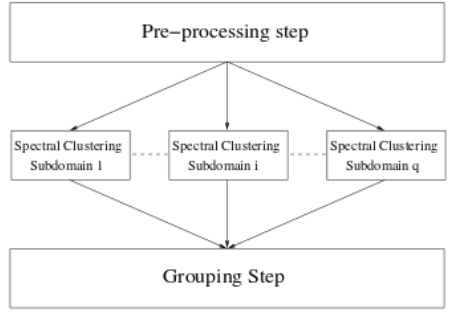
\includegraphics[width=0.5\linewidth]{Image/parallel.png}}
\caption{}
\label{fig:speciation}
\end{figure}



\section{Documentation}
The following reference can be used for any theoretical understanding of the algorithm. It also provides references on the minimum interface the different method must follow.

\begin{itemize}
\item The Global Kernel k-Means Clustering Algorithm
Grigorios Tzortzis and Aristidis Likas
\item The Variable Bandwidth Mean Shift and Data-Driven Scale Selection
Dorin Comaniciu
Visvanathan Ramesh 
Peter Meer
\item Mean Shift Analysis and Applications
Dorin Comaniciu
Peter Meer

\end{itemize}
